\documentclass[1p]{elsarticle_modified}
%\bibliographystyle{elsarticle-num}

%\usepackage[colorlinks]{hyperref}
%\usepackage{abbrmath_seonhwa} %\Abb, \Ascr, \Acal ,\Abf, \Afrak
\usepackage{amsfonts}
\usepackage{amssymb}
\usepackage{amsmath}
\usepackage{amsthm}
\usepackage{scalefnt}
\usepackage{amsbsy}
\usepackage{kotex}
\usepackage{caption}
\usepackage{subfig}
\usepackage{color}
\usepackage{graphicx}
\usepackage{xcolor} %% white, black, red, green, blue, cyan, magenta, yellow
\usepackage{float}
\usepackage{setspace}
\usepackage{hyperref}

\usepackage{tikz}
\usetikzlibrary{arrows}

\usepackage{multirow}
\usepackage{array} % fixed length table
\usepackage{hhline}

%%%%%%%%%%%%%%%%%%%%%
\makeatletter
\renewcommand*\env@matrix[1][\arraystretch]{%
	\edef\arraystretch{#1}%
	\hskip -\arraycolsep
	\let\@ifnextchar\new@ifnextchar
	\array{*\c@MaxMatrixCols c}}
\makeatother %https://tex.stackexchange.com/questions/14071/how-can-i-increase-the-line-spacing-in-a-matrix
%%%%%%%%%%%%%%%

\usepackage[normalem]{ulem}

\newcommand{\msout}[1]{\ifmmode\text{\sout{\ensuremath{#1}}}\else\sout{#1}\fi}
%SOURCE: \msout is \stkout macro in https://tex.stackexchange.com/questions/20609/strikeout-in-math-mode

\newcommand{\cancel}[1]{
	\ifmmode
	{\color{red}\msout{#1}}
	\else
	{\color{red}\sout{#1}}
	\fi
}

\newcommand{\add}[1]{
	{\color{blue}\uwave{#1}}
}

\newcommand{\replace}[2]{
	\ifmmode
	{\color{red}\msout{#1}}{\color{blue}\uwave{#2}}
	\else
	{\color{red}\sout{#1}}{\color{blue}\uwave{#2}}
	\fi
}

\newcommand{\Sol}{\mathcal{S}} %segment
\newcommand{\D}{D} %diagram
\newcommand{\A}{\mathcal{A}} %arc


%%%%%%%%%%%%%%%%%%%%%%%%%%%%%5 test

\def\sl{\operatorname{\textup{SL}}(2,\Cbb)}
\def\psl{\operatorname{\textup{PSL}}(2,\Cbb)}
\def\quan{\mkern 1mu \triangleright \mkern 1mu}

\theoremstyle{definition}
\newtheorem{thm}{Theorem}[section]
\newtheorem{prop}[thm]{Proposition}
\newtheorem{lem}[thm]{Lemma}
\newtheorem{ques}[thm]{Question}
\newtheorem{cor}[thm]{Corollary}
\newtheorem{defn}[thm]{Definition}
\newtheorem{exam}[thm]{Example}
\newtheorem{rmk}[thm]{Remark}
\newtheorem{alg}[thm]{Algorithm}

\newcommand{\I}{\sqrt{-1}}
\begin{document}

%\begin{frontmatter}
%
%\title{Boundary parabolic representations of knots up to 8 crossings}
%
%%% Group authors per affiliation:
%\author{Yunhi Cho} 
%\address{Department of Mathematics, University of Seoul, Seoul, Korea}
%\ead{yhcho@uos.ac.kr}
%
%
%\author{Seonhwa Kim} %\fnref{s_kim}}
%\address{Center for Geometry and Physics, Institute for Basic Science, Pohang, 37673, Korea}
%\ead{ryeona17@ibs.re.kr}
%
%\author{Hyuk Kim}
%\address{Department of Mathematical Sciences, Seoul National University, Seoul 08826, Korea}
%\ead{hyukkim@snu.ac.kr}
%
%\author{Seokbeom Yoon}
%\address{Department of Mathematical Sciences, Seoul National University, Seoul, 08826,  Korea}
%\ead{sbyoon15@snu.ac.kr}
%
%\begin{abstract}
%We find all boundary parabolic representation of knots up to 8 crossings.
%
%\end{abstract}
%\begin{keyword}
%    \MSC[2010] 57M25 
%\end{keyword}
%
%\end{frontmatter}

%\linenumbers
%\tableofcontents
%
\newcommand\colored[1]{\textcolor{white}{\rule[-0.35ex]{0.8em}{1.4ex}}\kern-0.8em\color{red} #1}%
%\newcommand\colored[1]{\textcolor{white}{ #1}\kern-2.17ex	\textcolor{white}{ #1}\kern-1.81ex	\textcolor{white}{ #1}\kern-2.15ex\color{red}#1	}

{\Large $\underline{11n_{26}~(K11n_{26})}$}

\setlength{\tabcolsep}{10pt}
\renewcommand{\arraystretch}{1.6}
\vspace{1cm}\begin{tabular}{m{100pt}>{\centering\arraybackslash}m{274pt}}
\multirow{5}{120pt}{
	\centering
	\includegraphics[width=112pt]{../../../GIT/diagram.site/Diagrams/png/642_11n_26.png}\\
\ \ \ A knot diagram\footnotemark}&
\allowdisplaybreaks
\textbf{Linearized knot diagam} \\
\cline{2-2}
 &
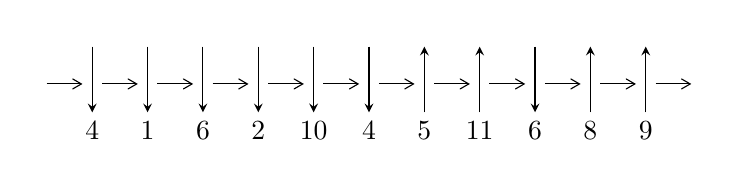
\begin{tikzpicture}[x=20pt, y=17pt]
	% nodes
	\node (C0) at (0, 0) {};
	\node (C1) at (1, 0) {};
	\node (C1U) at (1, +1) {};
	\node (C1D) at (1, -1) {4};

	\node (C2) at (2, 0) {};
	\node (C2U) at (2, +1) {};
	\node (C2D) at (2, -1) {1};

	\node (C3) at (3, 0) {};
	\node (C3U) at (3, +1) {};
	\node (C3D) at (3, -1) {6};

	\node (C4) at (4, 0) {};
	\node (C4U) at (4, +1) {};
	\node (C4D) at (4, -1) {2};

	\node (C5) at (5, 0) {};
	\node (C5U) at (5, +1) {};
	\node (C5D) at (5, -1) {10};

	\node (C6) at (6, 0) {};
	\node (C6U) at (6, +1) {};
	\node (C6D) at (6, -1) {4};

	\node (C7) at (7, 0) {};
	\node (C7U) at (7, +1) {};
	\node (C7D) at (7, -1) {5};

	\node (C8) at (8, 0) {};
	\node (C8U) at (8, +1) {};
	\node (C8D) at (8, -1) {11};

	\node (C9) at (9, 0) {};
	\node (C9U) at (9, +1) {};
	\node (C9D) at (9, -1) {6};

	\node (C10) at (10, 0) {};
	\node (C10U) at (10, +1) {};
	\node (C10D) at (10, -1) {8};

	\node (C11) at (11, 0) {};
	\node (C11U) at (11, +1) {};
	\node (C11D) at (11, -1) {9};
	\node (C12) at (12, 0) {};

	% arrows
	\draw[->,>={angle 60}]
	(C0) edge (C1) (C1) edge (C2) (C2) edge (C3) (C3) edge (C4) (C4) edge (C5) (C5) edge (C6) (C6) edge (C7) (C7) edge (C8) (C8) edge (C9) (C9) edge (C10) (C10) edge (C11) (C11) edge (C12) ;	\draw[->,>=stealth]
	(C1U) edge (C1D) (C2U) edge (C2D) (C3U) edge (C3D) (C4U) edge (C4D) (C5U) edge (C5D) (C6U) edge (C6D) (C7D) edge (C7U) (C8D) edge (C8U) (C9U) edge (C9D) (C10D) edge (C10U) (C11D) edge (C11U) ;
	\end{tikzpicture} \\
\hhline{~~} \\& 
\textbf{Solving Sequence} \\ \cline{2-2} 
 &
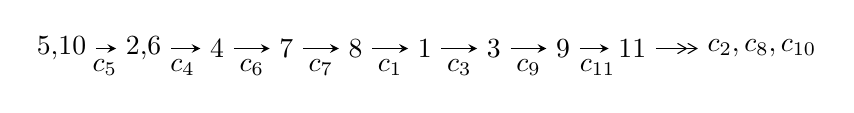
\begin{tikzpicture}[x=25pt, y=7pt]
	% node
	\node (A0) at (-1/8, 0) {5,10};
	\node (A1) at (17/16, 0) {2,6};
	\node (A2) at (17/8, 0) {4};
	\node (A3) at (25/8, 0) {7};
	\node (A4) at (33/8, 0) {8};
	\node (A5) at (41/8, 0) {1};
	\node (A6) at (49/8, 0) {3};
	\node (A7) at (57/8, 0) {9};
	\node (A8) at (65/8, 0) {11};
	\node (C1) at (1/2, -1) {$c_{5}$};
	\node (C2) at (13/8, -1) {$c_{4}$};
	\node (C3) at (21/8, -1) {$c_{6}$};
	\node (C4) at (29/8, -1) {$c_{7}$};
	\node (C5) at (37/8, -1) {$c_{1}$};
	\node (C6) at (45/8, -1) {$c_{3}$};
	\node (C7) at (53/8, -1) {$c_{9}$};
	\node (C8) at (61/8, -1) {$c_{11}$};
	\node (A9) at (10, 0) {$c_{2},c_{8},c_{10}$};

	% edge
	\draw[->,>=stealth]	
	(A0) edge (A1) (A1) edge (A2) (A2) edge (A3) (A3) edge (A4) (A4) edge (A5) (A5) edge (A6) (A6) edge (A7) (A7) edge (A8) ;
	\draw[->>,>={angle 60}]	
	(A8) edge (A9);
\end{tikzpicture} \\ 

\end{tabular} \\

\footnotetext{
The image of knot diagram is generated by the software ``\textbf{Draw programme}" developed by Andrew Bartholomew(\url{http://www.layer8.co.uk/maths/draw/index.htm\#Running-draw}), where we modified some parts for our purpose(\url{https://github.com/CATsTAILs/LinksPainter}).
}\phantom \\ \newline 
\centering \textbf{Ideals for irreducible components\footnotemark of $X_{\text{par}}$} 
 
\begin{align*}
I^u_{1}&=\langle 
6.49349\times10^{26} u^{27}+1.90286\times10^{27} u^{26}+\cdots+6.31630\times10^{27} b-6.60130\times10^{27},\\
\phantom{I^u_{1}}&\phantom{= \langle  }-1.10262\times10^{28} u^{27}-1.96649\times10^{28} u^{26}+\cdots+1.26326\times10^{28} a-2.28561\times10^{29},\\
\phantom{I^u_{1}}&\phantom{= \langle  }u^{28}+2 u^{27}+\cdots+20 u+8\rangle \\
I^u_{2}&=\langle 
b+1,\;u^4+u^2+a- u+1,\;u^5+u^4+2 u^3+u^2+u+1\rangle \\
\\
I^v_{1}&=\langle 
a,\;- v^2+b+3 v+1,\;v^3-2 v^2-3 v-1\rangle \\
\end{align*}
\raggedright * 3 irreducible components of $\dim_{\mathbb{C}}=0$, with total 36 representations.\\
\footnotetext{All coefficients of polynomials are rational numbers. But the coefficients are sometimes approximated in decimal forms when there is not enough margin.}
\newpage
\renewcommand{\arraystretch}{1}
\centering \section*{I. $I^u_{1}= \langle 6.49\times10^{26} u^{27}+1.90\times10^{27} u^{26}+\cdots+6.32\times10^{27} b-6.60\times10^{27},\;-1.10\times10^{28} u^{27}-1.97\times10^{28} u^{26}+\cdots+1.26\times10^{28} a-2.29\times10^{29},\;u^{28}+2 u^{27}+\cdots+20 u+8 \rangle$}
\flushleft \textbf{(i) Arc colorings}\\
\begin{tabular}{m{7pt} m{180pt} m{7pt} m{180pt} }
\flushright $a_{5}=$&$\begin{pmatrix}1\\0\end{pmatrix}$ \\
\flushright $a_{10}=$&$\begin{pmatrix}0\\u\end{pmatrix}$ \\
\flushright $a_{2}=$&$\begin{pmatrix}0.872833 u^{27}+1.55668 u^{26}+\cdots-6.74875 u+18.0929\\-0.102805 u^{27}-0.301262 u^{26}+\cdots+5.99581 u+1.04512\end{pmatrix}$ \\
\flushright $a_{6}=$&$\begin{pmatrix}1\\u^2\end{pmatrix}$ \\
\flushright $a_{4}=$&$\begin{pmatrix}0.748842 u^{27}+1.32169 u^{26}+\cdots-4.76990 u+17.3225\\0.236809 u^{27}+0.571914 u^{26}+\cdots-10.8084 u-2.70142\end{pmatrix}$ \\
\flushright $a_{7}=$&$\begin{pmatrix}0.212982 u^{27}+0.380557 u^{26}+\cdots-3.15104 u+3.02347\\-0.0259598 u^{27}-0.0939752 u^{26}+\cdots+1.35732 u+1.55242\end{pmatrix}$ \\
\flushright $a_{8}=$&$\begin{pmatrix}0.187022 u^{27}+0.286582 u^{26}+\cdots-1.79372 u+4.57588\\-0.0259598 u^{27}-0.0939752 u^{26}+\cdots+1.35732 u+1.55242\end{pmatrix}$ \\
\flushright $a_{1}=$&$\begin{pmatrix}0.212982 u^{27}+0.380557 u^{26}+\cdots-3.15104 u+3.02347\\0.0387264 u^{27}+0.130165 u^{26}+\cdots-2.15306 u-1.18917\end{pmatrix}$ \\
\flushright $a_{3}=$&$\begin{pmatrix}0.902672 u^{27}+1.78001 u^{26}+\cdots-13.1074 u+13.2132\\0.300350 u^{27}+0.747310 u^{26}+\cdots-15.0523 u-3.90671\end{pmatrix}$ \\
\flushright $a_{9}=$&$\begin{pmatrix}u\\u^3+u\end{pmatrix}$ \\
\flushright $a_{11}=$&$\begin{pmatrix}0.216279 u^{27}+0.376927 u^{26}+\cdots-2.89799 u+3.72316\\0.0537576 u^{27}+0.145064 u^{26}+\cdots-1.72187 u-0.407669\end{pmatrix}$\\ \flushright $a_{11}=$&$\begin{pmatrix}0.216279 u^{27}+0.376927 u^{26}+\cdots-2.89799 u+3.72316\\0.0537576 u^{27}+0.145064 u^{26}+\cdots-1.72187 u-0.407669\end{pmatrix}$\\&\end{tabular}
\flushleft \textbf{(ii) Obstruction class $= -1$}\\~\\
\flushleft \textbf{(iii) Cusp Shapes $= \frac{10054887119174523839900746713}{6316300717618506105858780668} u^{27}+\frac{3421814896803148511487522420}{1579075179404626526464695167} u^{26}+\cdots+\frac{38462222224803397140841081069}{3158150358809253052929390334} u+\frac{73867545823191868965381639557}{1579075179404626526464695167}$}\\~\\
\newpage\renewcommand{\arraystretch}{1}
\flushleft \textbf{(iv) u-Polynomials at the component}\newline \\
\begin{tabular}{m{50pt}|m{274pt}}
Crossings & \hspace{64pt}u-Polynomials at each crossing \\
\hline $$\begin{aligned}c_{1},c_{4}\end{aligned}$$&$\begin{aligned}
&u^{28}-7 u^{27}+\cdots-5 u+1
\end{aligned}$\\
\hline $$\begin{aligned}c_{2}\end{aligned}$$&$\begin{aligned}
&u^{28}+5 u^{27}+\cdots-3 u+1
\end{aligned}$\\
\hline $$\begin{aligned}c_{3},c_{6}\end{aligned}$$&$\begin{aligned}
&u^{28}-2 u^{27}+\cdots-24 u^2-32
\end{aligned}$\\
\hline $$\begin{aligned}c_{5},c_{9}\end{aligned}$$&$\begin{aligned}
&u^{28}+2 u^{27}+\cdots+20 u+8
\end{aligned}$\\
\hline $$\begin{aligned}c_{7}\end{aligned}$$&$\begin{aligned}
&u^{28}+3 u^{27}+\cdots- u-1
\end{aligned}$\\
\hline $$\begin{aligned}c_{8},c_{10},c_{11}\end{aligned}$$&$\begin{aligned}
&u^{28}+5 u^{27}+\cdots-8 u-1
\end{aligned}$\\
\hline
\end{tabular}\\~\\
\newpage\renewcommand{\arraystretch}{1}
\flushleft \textbf{(v) Riley Polynomials at the component}\newline \\
\begin{tabular}{m{50pt}|m{274pt}}
Crossings & \hspace{64pt}Riley Polynomials at each crossing \\
\hline $$\begin{aligned}c_{1},c_{4}\end{aligned}$$&$\begin{aligned}
&y^{28}-5 y^{27}+\cdots+3 y+1
\end{aligned}$\\
\hline $$\begin{aligned}c_{2}\end{aligned}$$&$\begin{aligned}
&y^{28}+43 y^{27}+\cdots+3 y+1
\end{aligned}$\\
\hline $$\begin{aligned}c_{3},c_{6}\end{aligned}$$&$\begin{aligned}
&y^{28}+36 y^{27}+\cdots+1536 y+1024
\end{aligned}$\\
\hline $$\begin{aligned}c_{5},c_{9}\end{aligned}$$&$\begin{aligned}
&y^{28}+24 y^{27}+\cdots-848 y+64
\end{aligned}$\\
\hline $$\begin{aligned}c_{7}\end{aligned}$$&$\begin{aligned}
&y^{28}-37 y^{27}+\cdots-35 y+1
\end{aligned}$\\
\hline $$\begin{aligned}c_{8},c_{10},c_{11}\end{aligned}$$&$\begin{aligned}
&y^{28}-31 y^{27}+\cdots-128 y+1
\end{aligned}$\\
\hline
\end{tabular}\\~\\
\newpage\flushleft \textbf{(vi) Complex Volumes and Cusp Shapes}
$$\begin{array}{c|c|c}  
\text{Solutions to }I^u_{1}& \I (\text{vol} + \sqrt{-1}CS) & \text{Cusp shape}\\
 \hline 
\begin{aligned}
u &= -0.502386 + 0.824854 I \\
a &= \phantom{-}0.823470 + 0.487809 I \\
b &= \phantom{-}0.414733 - 0.266521 I\end{aligned}
 & -0.04395 + 1.99045 I & -0.01306 - 4.61620 I \\ \hline\begin{aligned}
u &= -0.502386 - 0.824854 I \\
a &= \phantom{-}0.823470 - 0.487809 I \\
b &= \phantom{-}0.414733 + 0.266521 I\end{aligned}
 & -0.04395 - 1.99045 I & -0.01306 + 4.61620 I \\ \hline\begin{aligned}
u &= -0.011679 + 0.922740 I \\
a &= \phantom{-}0.91458 - 1.21166 I \\
b &= -0.220238 + 0.502777 I\end{aligned}
 & \phantom{-}1.30841 + 1.56433 I & \phantom{-}2.39227 - 4.63205 I \\ \hline\begin{aligned}
u &= -0.011679 - 0.922740 I \\
a &= \phantom{-}0.91458 + 1.21166 I \\
b &= -0.220238 - 0.502777 I\end{aligned}
 & \phantom{-}1.30841 - 1.56433 I & \phantom{-}2.39227 + 4.63205 I \\ \hline\begin{aligned}
u &= \phantom{-}0.841010 + 0.306823 I \\
a &= \phantom{-}0.495652 - 0.321293 I \\
b &= \phantom{-}0.136281 - 0.404052 I\end{aligned}
 & \phantom{-}2.62794 + 0.46347 I & \phantom{-}2.20728 + 0.53901 I \\ \hline\begin{aligned}
u &= \phantom{-}0.841010 - 0.306823 I \\
a &= \phantom{-}0.495652 + 0.321293 I \\
b &= \phantom{-}0.136281 + 0.404052 I\end{aligned}
 & \phantom{-}2.62794 - 0.46347 I & \phantom{-}2.20728 - 0.53901 I \\ \hline\begin{aligned}
u &= \phantom{-}0.456033 + 1.080380 I \\
a &= \phantom{-}0.760375 - 0.367537 I \\
b &= \phantom{-}0.744635 + 0.318856 I\end{aligned}
 & \phantom{-}4.82268 - 5.10002 I & \phantom{-}4.96882 + 7.61668 I \\ \hline\begin{aligned}
u &= \phantom{-}0.456033 - 1.080380 I \\
a &= \phantom{-}0.760375 + 0.367537 I \\
b &= \phantom{-}0.744635 - 0.318856 I\end{aligned}
 & \phantom{-}4.82268 + 5.10002 I & \phantom{-}4.96882 - 7.61668 I \\ \hline\begin{aligned}
u &= \phantom{-}0.639311 + 0.009558 I \\
a &= \phantom{-}0.530838 + 0.374755 I \\
b &= \phantom{-}0.894453 - 0.824309 I\end{aligned}
 & \phantom{-}3.90340 + 3.06304 I & -6.04954 - 3.66902 I \\ \hline\begin{aligned}
u &= \phantom{-}0.639311 - 0.009558 I \\
a &= \phantom{-}0.530838 - 0.374755 I \\
b &= \phantom{-}0.894453 + 0.824309 I\end{aligned}
 & \phantom{-}3.90340 - 3.06304 I & -6.04954 + 3.66902 I\\
 \hline 
 \end{array}$$\newpage$$\begin{array}{c|c|c}  
\text{Solutions to }I^u_{1}& \I (\text{vol} + \sqrt{-1}CS) & \text{Cusp shape}\\
 \hline 
\begin{aligned}
u &= \phantom{-}0.100025 + 0.630262 I \\
a &= \phantom{-}0.34419 + 2.12537 I \\
b &= -1.051400 - 0.149533 I\end{aligned}
 & -1.169040 - 0.736496 I & -2.56323 - 2.93619 I \\ \hline\begin{aligned}
u &= \phantom{-}0.100025 - 0.630262 I \\
a &= \phantom{-}0.34419 - 2.12537 I \\
b &= -1.051400 + 0.149533 I\end{aligned}
 & -1.169040 + 0.736496 I & -2.56323 + 2.93619 I \\ \hline\begin{aligned}
u &= -0.09653 + 1.44384 I \\
a &= -0.313167 - 0.868043 I \\
b &= -1.322620 + 0.396919 I\end{aligned}
 & \phantom{-}5.47968 + 1.56446 I & \phantom{-}1.30115 - 0.62804 I \\ \hline\begin{aligned}
u &= -0.09653 - 1.44384 I \\
a &= -0.313167 + 0.868043 I \\
b &= -1.322620 - 0.396919 I\end{aligned}
 & \phantom{-}5.47968 - 1.56446 I & \phantom{-}1.30115 + 0.62804 I \\ \hline\begin{aligned}
u &= \phantom{-}0.11027 + 1.45639 I \\
a &= -0.590568 + 1.231490 I \\
b &= \phantom{-}0.95494 - 1.07229 I\end{aligned}
 & \phantom{-}9.13873 + 0.66915 I & \phantom{-}1.241168 + 0.226691 I \\ \hline\begin{aligned}
u &= \phantom{-}0.11027 - 1.45639 I \\
a &= -0.590568 - 1.231490 I \\
b &= \phantom{-}0.95494 + 1.07229 I\end{aligned}
 & \phantom{-}9.13873 - 0.66915 I & \phantom{-}1.241168 - 0.226691 I \\ \hline\begin{aligned}
u &= \phantom{-}0.33116 + 1.43263 I \\
a &= -0.03375 - 1.59565 I \\
b &= \phantom{-}1.08042 + 0.99381 I\end{aligned}
 & \phantom{-}8.71794 - 6.87707 I & \phantom{-}0.35894 + 4.81213 I \\ \hline\begin{aligned}
u &= \phantom{-}0.33116 - 1.43263 I \\
a &= -0.03375 + 1.59565 I \\
b &= \phantom{-}1.08042 - 0.99381 I\end{aligned}
 & \phantom{-}8.71794 + 6.87707 I & \phantom{-}0.35894 - 4.81213 I \\ \hline\begin{aligned}
u &= -1.51203 + 0.11931 I \\
a &= \phantom{-}0.447872 - 0.348583 I \\
b &= \phantom{-}1.03272 + 1.05137 I\end{aligned}
 & \phantom{-}11.20710 - 3.83748 I & \phantom{-}1.59779 + 2.22620 I \\ \hline\begin{aligned}
u &= -1.51203 - 0.11931 I \\
a &= \phantom{-}0.447872 + 0.348583 I \\
b &= \phantom{-}1.03272 - 1.05137 I\end{aligned}
 & \phantom{-}11.20710 + 3.83748 I & \phantom{-}1.59779 - 2.22620 I\\
 \hline 
 \end{array}$$\newpage$$\begin{array}{c|c|c}  
\text{Solutions to }I^u_{1}& \I (\text{vol} + \sqrt{-1}CS) & \text{Cusp shape}\\
 \hline 
\begin{aligned}
u &= \phantom{-}0.29853 + 1.54812 I \\
a &= \phantom{-}0.139401 + 1.066540 I \\
b &= -0.423937 - 0.981765 I\end{aligned}
 & \phantom{-}8.83250 - 3.91759 I & \phantom{-}2.90293 + 3.10234 I \\ \hline\begin{aligned}
u &= \phantom{-}0.29853 - 1.54812 I \\
a &= \phantom{-}0.139401 - 1.066540 I \\
b &= -0.423937 + 0.981765 I\end{aligned}
 & \phantom{-}8.83250 + 3.91759 I & \phantom{-}2.90293 - 3.10234 I \\ \hline\begin{aligned}
u &= -0.349253\phantom{ +0.000000I} \\
a &= -12.0202\phantom{ +0.000000I} \\
b &= -0.917213\phantom{ +0.000000I}\end{aligned}
 & \phantom{-}0.303143\phantom{ +0.000000I} & -47.2620\phantom{ +0.000000I} \\ \hline\begin{aligned}
u &= -0.304533\phantom{ +0.000000I} \\
a &= \phantom{-}1.10498\phantom{ +0.000000I} \\
b &= -0.668462\phantom{ +0.000000I}\end{aligned}
 & -1.01341\phantom{ +0.000000I} & -10.2410\phantom{ +0.000000I} \\ \hline\begin{aligned}
u &= -0.72992 + 1.54911 I \\
a &= \phantom{-}0.43631 + 1.34583 I \\
b &= \phantom{-}1.21166 - 0.95824 I\end{aligned}
 & \phantom{-}15.7181 + 11.7289 I & \phantom{-}1.85525 - 5.52053 I \\ \hline\begin{aligned}
u &= -0.72992 - 1.54911 I \\
a &= \phantom{-}0.43631 - 1.34583 I \\
b &= \phantom{-}1.21166 + 0.95824 I\end{aligned}
 & \phantom{-}15.7181 - 11.7289 I & \phantom{-}1.85525 + 5.52053 I \\ \hline\begin{aligned}
u &= -0.59689 + 1.68228 I \\
a &= -0.497600 - 0.677471 I \\
b &= \phantom{-}0.84120 + 1.23310 I\end{aligned}
 & \phantom{-}16.9931 + 3.8383 I & \phantom{-0.000000 } 0 \\ \hline\begin{aligned}
u &= -0.59689 - 1.68228 I \\
a &= -0.497600 + 0.677471 I \\
b &= \phantom{-}0.84120 - 1.23310 I\end{aligned}
 & \phantom{-}16.9931 - 3.8383 I & \phantom{-0.000000 } 0\\
 \hline 
 \end{array}$$\newpage\newpage\renewcommand{\arraystretch}{1}
\centering \section*{II. $I^u_{2}= \langle b+1,\;u^4+u^2+a- u+1,\;u^5+u^4+2 u^3+u^2+u+1 \rangle$}
\flushleft \textbf{(i) Arc colorings}\\
\begin{tabular}{m{7pt} m{180pt} m{7pt} m{180pt} }
\flushright $a_{5}=$&$\begin{pmatrix}1\\0\end{pmatrix}$ \\
\flushright $a_{10}=$&$\begin{pmatrix}0\\u\end{pmatrix}$ \\
\flushright $a_{2}=$&$\begin{pmatrix}- u^4- u^2+u-1\\-1\end{pmatrix}$ \\
\flushright $a_{6}=$&$\begin{pmatrix}1\\u^2\end{pmatrix}$ \\
\flushright $a_{4}=$&$\begin{pmatrix}- u^4- u^2+u\\-1\end{pmatrix}$ \\
\flushright $a_{7}=$&$\begin{pmatrix}1\\u^2\end{pmatrix}$ \\
\flushright $a_{8}=$&$\begin{pmatrix}u^2+1\\u^2\end{pmatrix}$ \\
\flushright $a_{1}=$&$\begin{pmatrix}-1\\0\end{pmatrix}$ \\
\flushright $a_{3}=$&$\begin{pmatrix}- u^4- u^2+u\\-1\end{pmatrix}$ \\
\flushright $a_{9}=$&$\begin{pmatrix}u\\u^3+u\end{pmatrix}$ \\
\flushright $a_{11}=$&$\begin{pmatrix}- u^4- u^2-1\\- u^4- u^3- u^2-1\end{pmatrix}$\\ \flushright $a_{11}=$&$\begin{pmatrix}- u^4- u^2-1\\- u^4- u^3- u^2-1\end{pmatrix}$\\&\end{tabular}
\flushleft \textbf{(ii) Obstruction class $= 1$}\\~\\
\flushleft \textbf{(iii) Cusp Shapes $= 2 u^4+5 u^3+7 u^2+5 u$}\\~\\
\newpage\renewcommand{\arraystretch}{1}
\flushleft \textbf{(iv) u-Polynomials at the component}\newline \\
\begin{tabular}{m{50pt}|m{274pt}}
Crossings & \hspace{64pt}u-Polynomials at each crossing \\
\hline $$\begin{aligned}c_{1}\end{aligned}$$&$\begin{aligned}
&(u-1)^5
\end{aligned}$\\
\hline $$\begin{aligned}c_{2},c_{4}\end{aligned}$$&$\begin{aligned}
&(u+1)^5
\end{aligned}$\\
\hline $$\begin{aligned}c_{3},c_{6}\end{aligned}$$&$\begin{aligned}
&u^5
\end{aligned}$\\
\hline $$\begin{aligned}c_{5}\end{aligned}$$&$\begin{aligned}
&u^5+u^4+2 u^3+u^2+u+1
\end{aligned}$\\
\hline $$\begin{aligned}c_{7}\end{aligned}$$&$\begin{aligned}
&u^5-3 u^4+4 u^3- u^2- u+1
\end{aligned}$\\
\hline $$\begin{aligned}c_{8}\end{aligned}$$&$\begin{aligned}
&u^5- u^4-2 u^3+u^2+u+1
\end{aligned}$\\
\hline $$\begin{aligned}c_{9}\end{aligned}$$&$\begin{aligned}
&u^5- u^4+2 u^3- u^2+u-1
\end{aligned}$\\
\hline $$\begin{aligned}c_{10},c_{11}\end{aligned}$$&$\begin{aligned}
&u^5+u^4-2 u^3- u^2+u-1
\end{aligned}$\\
\hline
\end{tabular}\\~\\
\newpage\renewcommand{\arraystretch}{1}
\flushleft \textbf{(v) Riley Polynomials at the component}\newline \\
\begin{tabular}{m{50pt}|m{274pt}}
Crossings & \hspace{64pt}Riley Polynomials at each crossing \\
\hline $$\begin{aligned}c_{1},c_{2},c_{4}\end{aligned}$$&$\begin{aligned}
&(y-1)^5
\end{aligned}$\\
\hline $$\begin{aligned}c_{3},c_{6}\end{aligned}$$&$\begin{aligned}
&y^5
\end{aligned}$\\
\hline $$\begin{aligned}c_{5},c_{9}\end{aligned}$$&$\begin{aligned}
&y^5+3 y^4+4 y^3+y^2- y-1
\end{aligned}$\\
\hline $$\begin{aligned}c_{7}\end{aligned}$$&$\begin{aligned}
&y^5- y^4+8 y^3-3 y^2+3 y-1
\end{aligned}$\\
\hline $$\begin{aligned}c_{8},c_{10},c_{11}\end{aligned}$$&$\begin{aligned}
&y^5-5 y^4+8 y^3-3 y^2- y-1
\end{aligned}$\\
\hline
\end{tabular}\\~\\
\newpage\flushleft \textbf{(vi) Complex Volumes and Cusp Shapes}
$$\begin{array}{c|c|c}  
\text{Solutions to }I^u_{2}& \I (\text{vol} + \sqrt{-1}CS) & \text{Cusp shape}\\
 \hline 
\begin{aligned}
u &= \phantom{-}0.339110 + 0.822375 I \\
a &= -0.103562 + 0.890762 I \\
b &= -1.00000\phantom{ +0.000000I}\end{aligned}
 & -1.31583 - 1.53058 I & -5.47076 + 5.40154 I \\ \hline\begin{aligned}
u &= \phantom{-}0.339110 - 0.822375 I \\
a &= -0.103562 - 0.890762 I \\
b &= -1.00000\phantom{ +0.000000I}\end{aligned}
 & -1.31583 + 1.53058 I & -5.47076 - 5.40154 I \\ \hline\begin{aligned}
u &= -0.766826\phantom{ +0.000000I} \\
a &= -2.70062\phantom{ +0.000000I} \\
b &= -1.00000\phantom{ +0.000000I}\end{aligned}
 & \phantom{-}0.756147\phantom{ +0.000000I} & -1.28100\phantom{ +0.000000I} \\ \hline\begin{aligned}
u &= -0.455697 + 1.200150 I \\
a &= -0.546130 - 0.402731 I \\
b &= -1.00000\phantom{ +0.000000I}\end{aligned}
 & \phantom{-}4.22763 + 4.40083 I & -0.88874 - 1.16747 I \\ \hline\begin{aligned}
u &= -0.455697 - 1.200150 I \\
a &= -0.546130 + 0.402731 I \\
b &= -1.00000\phantom{ +0.000000I}\end{aligned}
 & \phantom{-}4.22763 - 4.40083 I & -0.88874 + 1.16747 I\\
 \hline 
 \end{array}$$\newpage\newpage\renewcommand{\arraystretch}{1}
\centering \section*{III. $I^v_{1}= \langle a,\;- v^2+b+3 v+1,\;v^3-2 v^2-3 v-1 \rangle$}
\flushleft \textbf{(i) Arc colorings}\\
\begin{tabular}{m{7pt} m{180pt} m{7pt} m{180pt} }
\flushright $a_{5}=$&$\begin{pmatrix}1\\0\end{pmatrix}$ \\
\flushright $a_{10}=$&$\begin{pmatrix}v\\0\end{pmatrix}$ \\
\flushright $a_{2}=$&$\begin{pmatrix}0\\v^2-3 v-1\end{pmatrix}$ \\
\flushright $a_{6}=$&$\begin{pmatrix}1\\0\end{pmatrix}$ \\
\flushright $a_{4}=$&$\begin{pmatrix}1\\-2 v^2+5 v+3\end{pmatrix}$ \\
\flushright $a_{7}=$&$\begin{pmatrix}-2 v^2+5 v+4\\v^2-2 v-3\end{pmatrix}$ \\
\flushright $a_{8}=$&$\begin{pmatrix}- v^2+3 v+1\\v^2-2 v-3\end{pmatrix}$ \\
\flushright $a_{1}=$&$\begin{pmatrix}v^2-3 v-1\\- v^2+2 v+3\end{pmatrix}$ \\
\flushright $a_{3}=$&$\begin{pmatrix}-2 v^2+5 v+4\\-2 v^2+5 v+3\end{pmatrix}$ \\
\flushright $a_{9}=$&$\begin{pmatrix}v\\0\end{pmatrix}$ \\
\flushright $a_{11}=$&$\begin{pmatrix}v^2-2 v-1\\- v^2+2 v+3\end{pmatrix}$\\ \flushright $a_{11}=$&$\begin{pmatrix}v^2-2 v-1\\- v^2+2 v+3\end{pmatrix}$\\&\end{tabular}
\flushleft \textbf{(ii) Obstruction class $= 1$}\\~\\
\flushleft \textbf{(iii) Cusp Shapes $= 2 v^2-5 v+1$}\\~\\
\newpage\renewcommand{\arraystretch}{1}
\flushleft \textbf{(iv) u-Polynomials at the component}\newline \\
\begin{tabular}{m{50pt}|m{274pt}}
Crossings & \hspace{64pt}u-Polynomials at each crossing \\
\hline $$\begin{aligned}c_{1}\end{aligned}$$&$\begin{aligned}
&u^3+u^2-1
\end{aligned}$\\
\hline $$\begin{aligned}c_{2},c_{6}\end{aligned}$$&$\begin{aligned}
&u^3+u^2+2 u+1
\end{aligned}$\\
\hline $$\begin{aligned}c_{3}\end{aligned}$$&$\begin{aligned}
&u^3- u^2+2 u-1
\end{aligned}$\\
\hline $$\begin{aligned}c_{4}\end{aligned}$$&$\begin{aligned}
&u^3- u^2+1
\end{aligned}$\\
\hline $$\begin{aligned}c_{5},c_{9}\end{aligned}$$&$\begin{aligned}
&u^3
\end{aligned}$\\
\hline $$\begin{aligned}c_{7}\end{aligned}$$&$\begin{aligned}
&u^3-3 u^2+2 u+1
\end{aligned}$\\
\hline $$\begin{aligned}c_{8}\end{aligned}$$&$\begin{aligned}
&(u+1)^3
\end{aligned}$\\
\hline $$\begin{aligned}c_{10},c_{11}\end{aligned}$$&$\begin{aligned}
&(u-1)^3
\end{aligned}$\\
\hline
\end{tabular}\\~\\
\newpage\renewcommand{\arraystretch}{1}
\flushleft \textbf{(v) Riley Polynomials at the component}\newline \\
\begin{tabular}{m{50pt}|m{274pt}}
Crossings & \hspace{64pt}Riley Polynomials at each crossing \\
\hline $$\begin{aligned}c_{1},c_{4}\end{aligned}$$&$\begin{aligned}
&y^3- y^2+2 y-1
\end{aligned}$\\
\hline $$\begin{aligned}c_{2},c_{3},c_{6}\end{aligned}$$&$\begin{aligned}
&y^3+3 y^2+2 y-1
\end{aligned}$\\
\hline $$\begin{aligned}c_{5},c_{9}\end{aligned}$$&$\begin{aligned}
&y^3
\end{aligned}$\\
\hline $$\begin{aligned}c_{7}\end{aligned}$$&$\begin{aligned}
&y^3-5 y^2+10 y-1
\end{aligned}$\\
\hline $$\begin{aligned}c_{8},c_{10},c_{11}\end{aligned}$$&$\begin{aligned}
&(y-1)^3
\end{aligned}$\\
\hline
\end{tabular}\\~\\
\newpage\flushleft \textbf{(vi) Complex Volumes and Cusp Shapes}
$$\begin{array}{c|c|c}  
\text{Solutions to }I^v_{1}& \I (\text{vol} + \sqrt{-1}CS) & \text{Cusp shape}\\
 \hline 
\begin{aligned}
v &= -0.539798 + 0.182582 I \\
a &= \phantom{-0.000000 } 0 \\
b &= \phantom{-}0.877439 - 0.744862 I\end{aligned}
 & \phantom{-}4.66906 + 2.82812 I & \phantom{-}4.21508 - 1.30714 I \\ \hline\begin{aligned}
v &= -0.539798 - 0.182582 I \\
a &= \phantom{-0.000000 } 0 \\
b &= \phantom{-}0.877439 + 0.744862 I\end{aligned}
 & \phantom{-}4.66906 - 2.82812 I & \phantom{-}4.21508 + 1.30714 I \\ \hline\begin{aligned}
v &= \phantom{-}3.07960\phantom{ +0.000000I} \\
a &= \phantom{-0.000000 } 0 \\
b &= -0.754878\phantom{ +0.000000I}\end{aligned}
 & \phantom{-}0.531480\phantom{ +0.000000I} & \phantom{-}4.56980\phantom{ +0.000000I}\\
 \hline 
 \end{array}$$\newpage
\newpage\renewcommand{\arraystretch}{1}
\centering \section*{ IV. u-Polynomials}
\begin{tabular}{m{50pt}|m{274pt}}
Crossings & \hspace{64pt}u-Polynomials at each crossing \\
\hline $$\begin{aligned}c_{1}\end{aligned}$$&$\begin{aligned}
&((u-1)^5)(u^3+u^2-1)(u^{28}-7 u^{27}+\cdots-5 u+1)
\end{aligned}$\\
\hline $$\begin{aligned}c_{2}\end{aligned}$$&$\begin{aligned}
&((u+1)^5)(u^3+u^2+2 u+1)(u^{28}+5 u^{27}+\cdots-3 u+1)
\end{aligned}$\\
\hline $$\begin{aligned}c_{3}\end{aligned}$$&$\begin{aligned}
&u^5(u^3- u^2+2 u-1)(u^{28}-2 u^{27}+\cdots-24 u^2-32)
\end{aligned}$\\
\hline $$\begin{aligned}c_{4}\end{aligned}$$&$\begin{aligned}
&((u+1)^5)(u^3- u^2+1)(u^{28}-7 u^{27}+\cdots-5 u+1)
\end{aligned}$\\
\hline $$\begin{aligned}c_{5}\end{aligned}$$&$\begin{aligned}
&u^3(u^5+u^4+\cdots+u+1)(u^{28}+2 u^{27}+\cdots+20 u+8)
\end{aligned}$\\
\hline $$\begin{aligned}c_{6}\end{aligned}$$&$\begin{aligned}
&u^5(u^3+u^2+2 u+1)(u^{28}-2 u^{27}+\cdots-24 u^2-32)
\end{aligned}$\\
\hline $$\begin{aligned}c_{7}\end{aligned}$$&$\begin{aligned}
&(u^3-3 u^2+2 u+1)(u^5-3 u^4+\cdots- u+1)(u^{28}+3 u^{27}+\cdots- u-1)
\end{aligned}$\\
\hline $$\begin{aligned}c_{8}\end{aligned}$$&$\begin{aligned}
&((u+1)^3)(u^5- u^4+\cdots+u+1)(u^{28}+5 u^{27}+\cdots-8 u-1)
\end{aligned}$\\
\hline $$\begin{aligned}c_{9}\end{aligned}$$&$\begin{aligned}
&u^3(u^5- u^4+\cdots+u-1)(u^{28}+2 u^{27}+\cdots+20 u+8)
\end{aligned}$\\
\hline $$\begin{aligned}c_{10},c_{11}\end{aligned}$$&$\begin{aligned}
&((u-1)^3)(u^5+u^4+\cdots+u-1)(u^{28}+5 u^{27}+\cdots-8 u-1)
\end{aligned}$\\
\hline
\end{tabular}\newpage\renewcommand{\arraystretch}{1}
\centering \section*{ V. Riley Polynomials}
\begin{tabular}{m{50pt}|m{274pt}}
Crossings & \hspace{64pt}Riley Polynomials at each crossing \\
\hline $$\begin{aligned}c_{1},c_{4}\end{aligned}$$&$\begin{aligned}
&((y-1)^5)(y^3- y^2+2 y-1)(y^{28}-5 y^{27}+\cdots+3 y+1)
\end{aligned}$\\
\hline $$\begin{aligned}c_{2}\end{aligned}$$&$\begin{aligned}
&((y-1)^5)(y^3+3 y^2+2 y-1)(y^{28}+43 y^{27}+\cdots+3 y+1)
\end{aligned}$\\
\hline $$\begin{aligned}c_{3},c_{6}\end{aligned}$$&$\begin{aligned}
&y^5(y^3+3 y^2+2 y-1)(y^{28}+36 y^{27}+\cdots+1536 y+1024)
\end{aligned}$\\
\hline $$\begin{aligned}c_{5},c_{9}\end{aligned}$$&$\begin{aligned}
&y^3(y^5+3 y^4+\cdots- y-1)(y^{28}+24 y^{27}+\cdots-848 y+64)
\end{aligned}$\\
\hline $$\begin{aligned}c_{7}\end{aligned}$$&$\begin{aligned}
&(y^3-5 y^2+10 y-1)(y^5- y^4+8 y^3-3 y^2+3 y-1)\\
&\cdot(y^{28}-37 y^{27}+\cdots-35 y+1)
\end{aligned}$\\
\hline $$\begin{aligned}c_{8},c_{10},c_{11}\end{aligned}$$&$\begin{aligned}
&((y-1)^3)(y^5-5 y^4+\cdots- y-1)(y^{28}-31 y^{27}+\cdots-128 y+1)
\end{aligned}$\\
\hline
\end{tabular}
\vskip 2pc
\end{document}